\documentclass[12pt, a4paper, onecolumn]{article}
\usepackage{fontspec}
\usepackage{titlesec}
\usepackage[english]{babel}
\usepackage{blindtext}
\usepackage{subfig}
\usepackage{pgf}

\setmainfont{Georgia}
\titleformat{\section}
{\normalfont\fontspec{Arial}\fontsize{20pt}{0}\bfseries}
{\thesection}{20pt}{}

\begin{document}

\section{Theoretical Background}
	
	\paragraph{The physics of falling} have been researched on several occasions and the results can be read in a multitude of scientific papers and reports. Much of the research done in this area tries to distinguish the characteristics of a fall in comparison to other motional patterns conducted on a daily basis. For a fall detection system to be considered as reliable it is imperative that it has the means to separate actual fall accidents from other patterns resulting from activities of daily living (further referenced as ADL) to a fair extent. The earth's gravitational pull produces a constant acceleration by 9.8s m/$s^{2}$ towards the ground. This constant acceleration is also referenced as \textit{1g}. A fall would towards the earth's surface would thus initially mean a decrease in acceleration with respect to this natural constant, followed by a rapid acceleration in the other direction as the device (and possibly the person wearing it) hits either the ground or another surface.
	

	\paragraph{} Yildirim et. al takes a general approach to describe the character of several motional types \cite{int_journ}. In their research, they measured the response from a LSM330DLC acceleration sensor located in an Android device. Their approach uses a threshold value to indicate whether the acceleration vector exceeds the allowed limit for a crash. The blue, red and green lines corresponds to the acceleration on any of the three perpendicular axis \textit{X}, \textit{Y} and \textit{Z} shown below.
	
		\begin{figure}[h]
			\centering
			\subfloat{{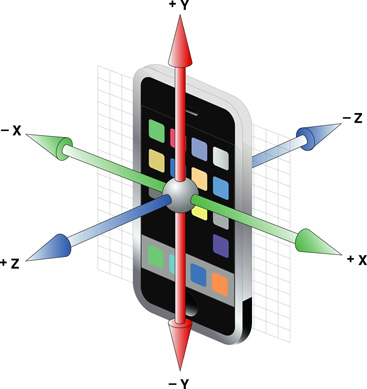
\includegraphics[width=8cm]{../img/accelerometer-axis.jpg} }}%
			\caption{The X, Y and Z axis af a smart phone device}%
			\label{fig:example}% 
		\end{figure}
	
		\begin{figure}[h]
			\centering
			\subfloat{{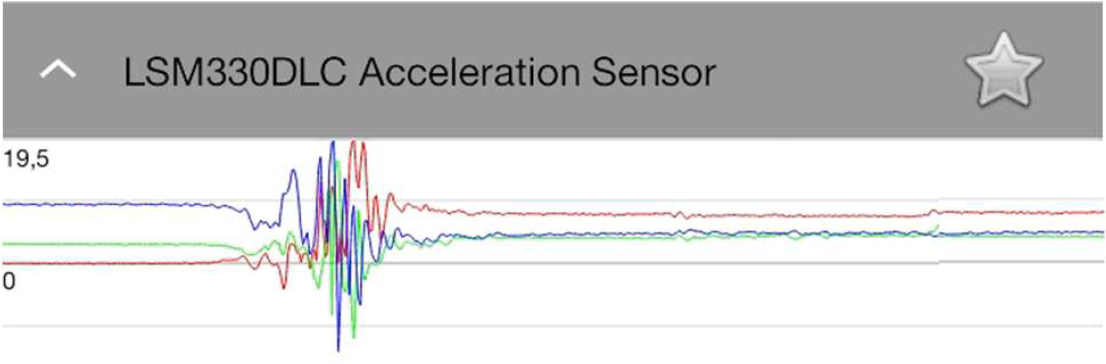
\includegraphics[width=8cm]{../img/Falling.png} }}%
			\caption{The typical pattern of falling}%
			\label{fig:example}%
		\end{figure}
	
		\noindent This measurements shows that falling, as was previously theorized, is indicated by a significant drop in acceleration towards the earth's gravitational pull, signaling that the device is moving towards a free fall state.This drop is then followed by an acceleration spike as the device hits the ground. If a person were to get seriously injured due to a fall s/he would usually remain still on the ground for a period of time. Acceleration would thus gradually go back to the normal \textit{1g} indicated by the flat line after the peak. 
	
	
		\begin{figure}[h]
			\centering
			\subfloat{{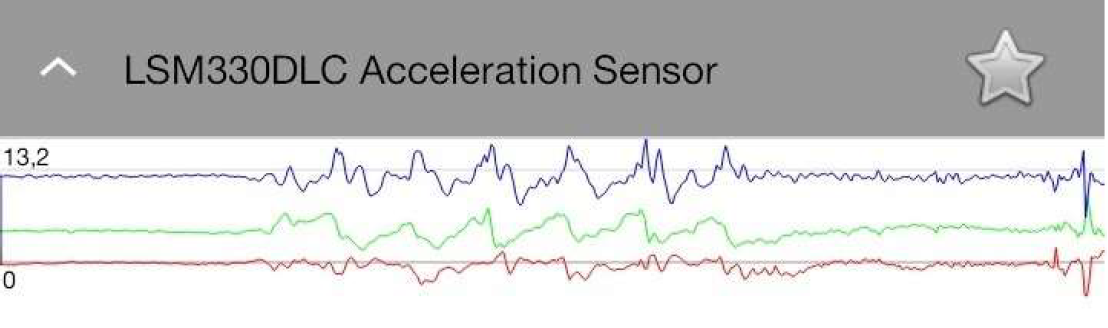
\includegraphics[width=8cm]{../img/Walking.png} }}%
			\caption{The typical pattern of walking}%
			\label{fig:example}%
		\end{figure}
	
		\noindent Walking shows a completely different pattern. As can be seen, the changes in acceleration are not rapid like the previous example. They are also repetitive, meaning that there is no longer period of non-movements after any of the peaks. The peaks them selves are also significant less than in the case of falling shown above. This implies that walking is easily distinguished from falling.
	
	
	
		\begin{figure}[h]
			\centering
			\subfloat{{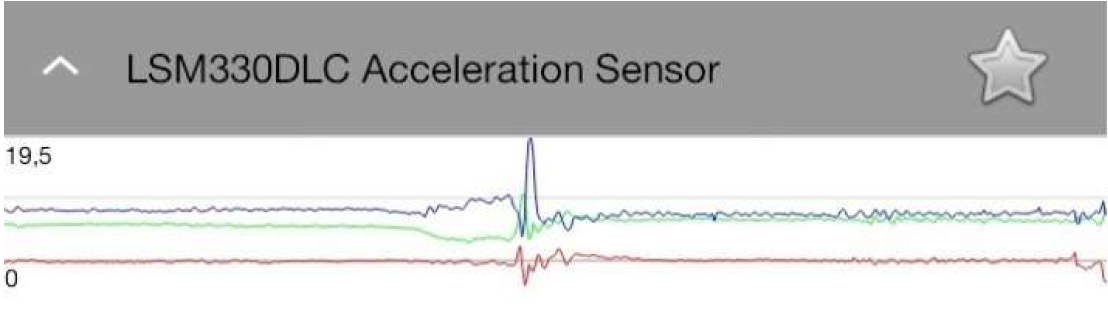
\includegraphics[width=8cm]{../img/Sitting_down.png} }}%
			\caption{The typical pattern of sitting down}%
			\label{fig:example}%
		\end{figure}
	
		\noindent Sitting down on a surface shows a similar pattern to falling with regards to a sudden drop in acceleration followed by  a rapid spike and a longer period of non-movement. The magnitude of these values are however far less than in the case of a fall and should thus be easy to single out. When a person sits down, s/he usually makes a soft movement towards the surface which is matched by the lesser accelerational  magnitude in all three directions \textit{X, Y} and \textit{Z}.
	
	
		\begin{figure}[h]
			\centering
			\subfloat{{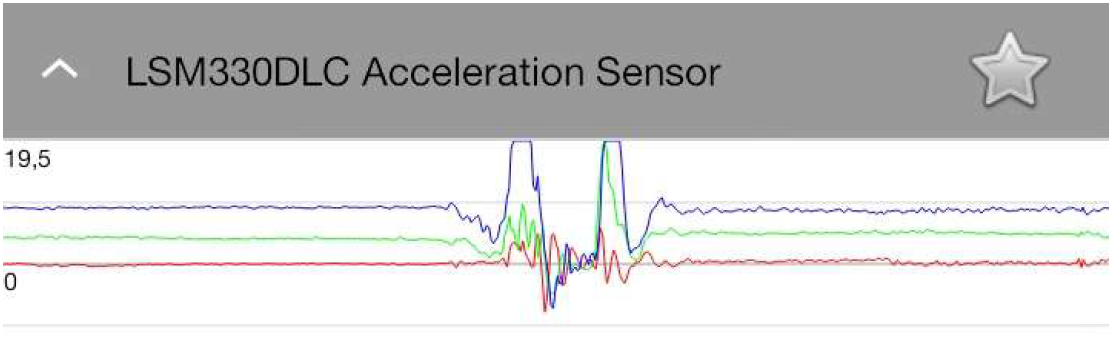
\includegraphics[width=8cm]{../img/Jumping.png} }}%
			\caption{The typical pattern of jumping}%
			\label{fig:example}%
		\end{figure}
	
		\noindent Jumping is according to Yildirim et. al. the hardest pattern to distinguish from a fall. The pattern has a sudden drop in acceleration, followed by a large spike as the jumper crouches and accelerates upwards. After this comes yet another sudden drop in acceleration as the jumper reaches the maximum altitude and starts falling back to earth again. From this part the pattern is almost identical to that of falling. When the jumper falls back to earth, the acceleration drops and then causes another huge spike as s/he hits the ground. When thinking about it, jumping and falling are in fact similar motional types, with the difference that jumping is prefixed by a drop and a spike before becoming an actual fall. The main challenge here is thus to be able to differentiate this from an unintentional falling accident.
		
		
		\paragraph{} Abbatea et. al. takes the above approach further by trying to establish a more sophisticated algorithm that utilizes more than merely just an acceleration vector compared to a threshold value to distinguish a fall like motional pattern from other types of ADL. Their thesis rely on several guidelines which among other include: 
			\begin{itemize} 
				\item "Detection of falls should be carried out using only acceleration-based information. Previous work demonstrated that acceleration is the most reliable information that can be used in detecting a fall, while other kinematic data, such as angular velocity, is less relevant." \cite[p~3]{piza_uni}
				
				\item "Still for usability reasons, the fall detection algorithm should work only with the magnitude of acceleration and not with the values along each of the three accelerometer’s axes, as this, again, would require a known and fixed orientation of the device with respect to the user’s body." \cite[p~3]{piza_uni}
			\end{itemize}
		
		The latter identifies the importance of calculating the resultant vector that comprises the sum of all three vectors \textit{X}, \textit{Y} and \textit{Z}. This vector is the overall acceleration imposed on the device (and possibly the person carrying it). They proceed by defining a \textit{fall-like-event} as "an acceleration greater than \textit{3g} followed by a period of \textit{2500ms} without further peaks exceeding the threshold." \cite[p~5]{piza_uni}. They further argue that the threshold \textit{3g} is chosen since it has been widely used in other types of fall detection systems. According to their experiments, a post-fall event usually means that the body of the unfortunate becomes lying still on the ground after a period of about \textit{1000ms}. This interval, which resides within the \textit{2500ms} interval prior to fall detection is often due to minor peaks following the main impact as a result of that parts of the body/device may hit the ground at different times. 
		
		\paragraph{} Abbatea et. al. tries to establish their algorithm using a \textit{finite-state-machine} with five distinct states. The \textit{sampling} state is the normal state that the process resides in until \textit{threshold-peak} is detected. 

		

	
\newpage


\bibliography{bib_peter}
\bibliographystyle{ieeetr}

\end{document}